In this section, we introduce key terms and concepts, utilised in our experiments. We cover additional knowledge, needed for understanding the applied methods. 
\subsection{EEG}
EEG is a non-invasive brain monitoring technique used to record electrical activity generated by neurons firing in the brain. The recording is usually executed via metal electrodes (such as silver, gold, or tin) placed on the scalp. EEG provides excellent temporal resolution – it can detect electrical changes in the brain on the order of milliseconds. This makes it appropriate for tracking rapid changes in brain dynamics. The recorded signals contain brain activity across distinct frequency bands (\cite{KUMAR20122525}, \cite{EEG_wavelengths}), each linked to specific cognitive and physiological states:
\begin{itemize}
    \item \textbf{Delta waves} (0.5–4 Hz): Linked to deep sleep.
    \item \textbf{Theta waves} (4–8 Hz): Associated with subconscious activities.
    \item \textbf{Alpha waves} (8–13 Hz): During states of relaxed wakefulness and are most pronounced in the further back regions of the head.
    \item \textbf{Beta waves} (13–30 Hz): Linked to active thinking, increased alertness, and anxiety.
    \item \textbf{Gamma waves} (30+ Hz): Indicate information processing and the commencement of voluntary movements.
\end{itemize}
Recording and working with EEG data poses significant challenges due to high dimensionality and high sensitivity to noise. Multiple electrodes record multiple signals simultaneously, thus resulting in high dimensionality and requiring significant computing power to analyse (\cite{10.1093/bioinformatics/btaf109}). Additionally, EEG signals are highly susceptible to noise and artefacts from both internal sources (such as eye blinks and muscle movements) and external sources (electrical interference), giving them a low signal-to-noise ratio. EEG has limited spatial resolution, making it difficult to pinpoint exact activity sources within the brain. Due to these factors, machine learning techniques become necessary for effective EEG analysis (\cite{Craik_2019}).
\begin{figure}
    \centering
    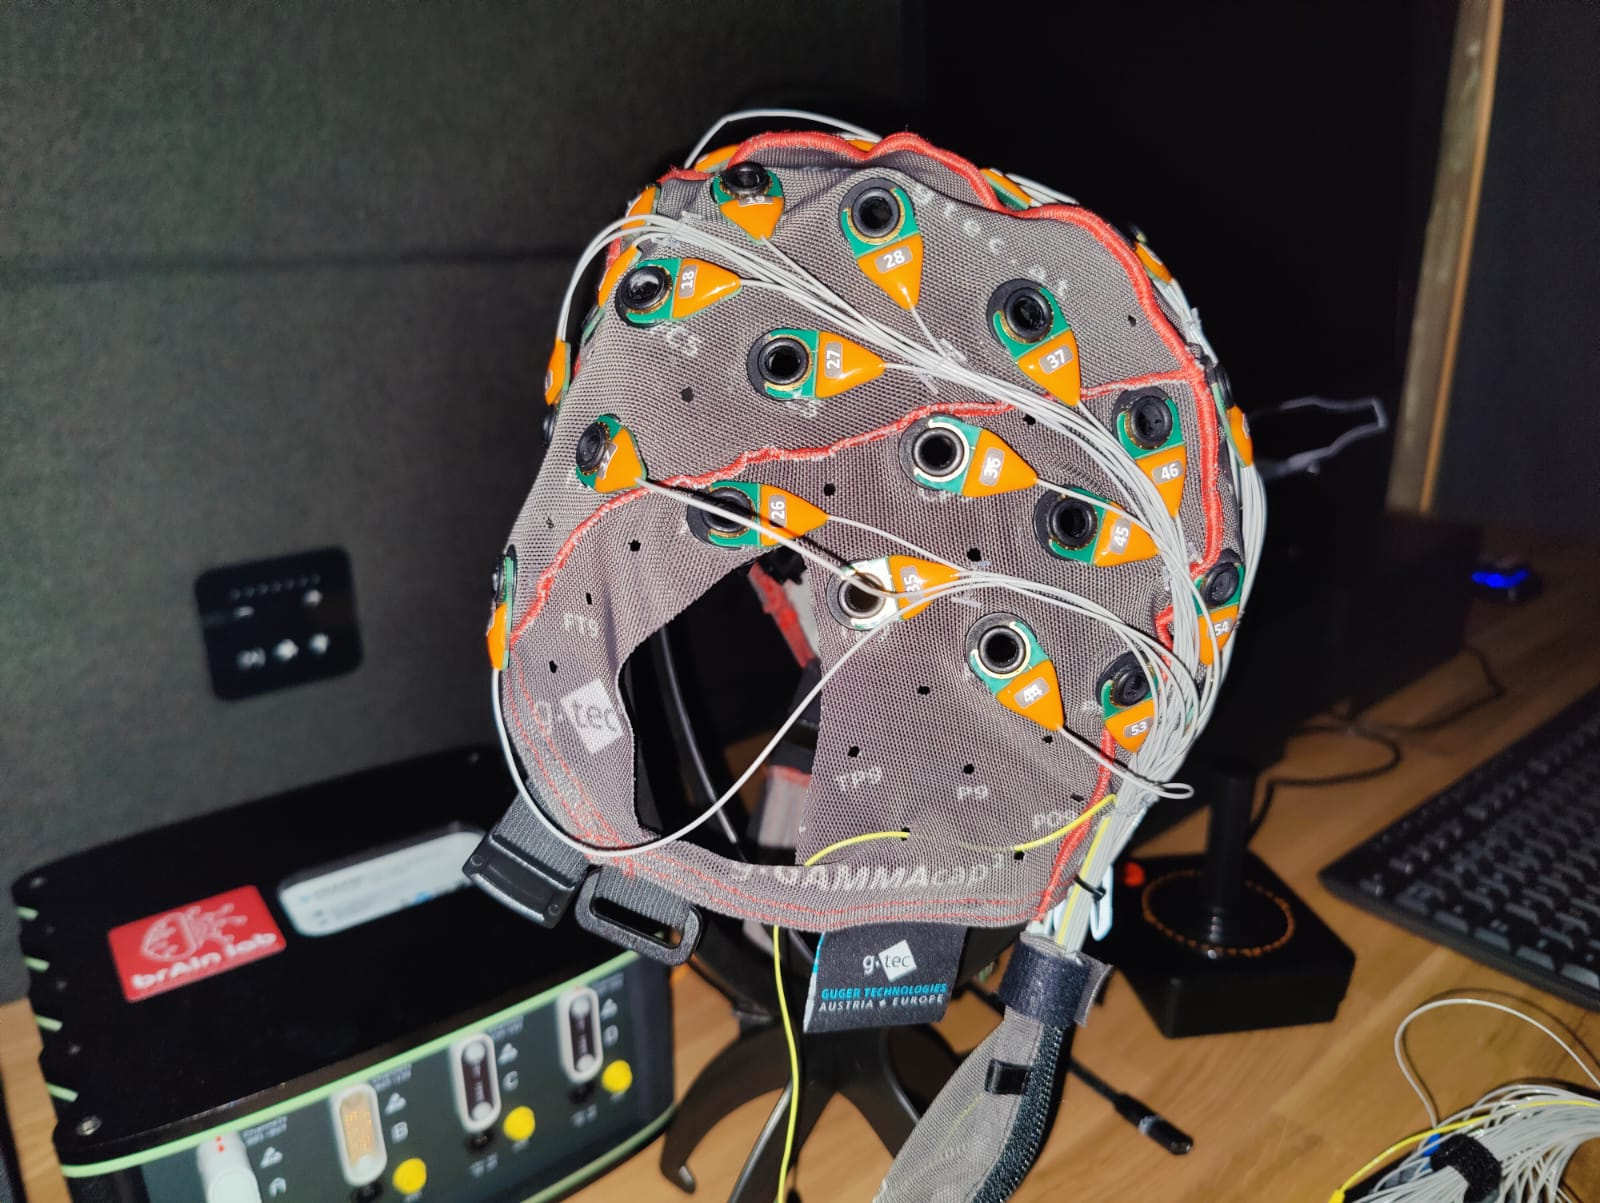
\includegraphics[width=0.5\linewidth]{img/eeg_cap.jpg}
    \caption{Example EEG capturing device from brAInlab at the IT University of Copenhagen. Seen here are electrodes placed according to the 10-20 system. This capturing device has more electrodes than the one used in this project.}
   % \caption{EEG capturing device from brAInlab at the IT University of Copenhagen. Electrode configuration differs from the one in the dataset used in this project.}
    \label{fig:enter-label}
\end{figure}
\subsection{EEG as a Data Type}
The aforementioned high dimensionality and noise sensitivity difficulties are further amplified in motor imagery tasks, where participants imagine movements rather than physically performing them, resulting in subtle neural signals that are harder to detect and classify.
\vspace{0.5em}\\
The EEG data used in this study were recorded using 22 Ag/AgCl electrodes placed according to the international 10–20 system, a widely adopted standard that positions electrodes at 10\% or 20\% intervals between anatomical landmarks such as the nasion (indentation between forehead and nose), inion (rear lower part of the skull), and preauricular points (in front of the ears). This system ensures consistent and reproducible electrode placement across different experiments and provides balanced coverage of cortical areas. The electrodes in our dataset – including Fz, FCz, Cz, Pz, POz along the midline, and FC3/4, C3/4, C1/2, C5/6, CP3/4, CP1, CPz, P1/2  – are symmetrically distributed across the scalp, odd-numbered electrodes on the left and even on the right side. This layout enables the monitoring of activity across frontal (F), frontocentral (FC), central (C), centroparietal (CP), parietal (P), and parieto-occipital (PO) regions, with a particular focus on sensorimotor areas that are especially relevant for motor imagery and cognitive processing.
%GNN
\subsection{Graph Neural Network}
GNNs are a class of deep learning models specifically designed to work with graph-structured data, using specialized convolution operations that can handle non-grid-like structures.(\cite{GNNBook}).
\vspace{0.5em}\\
The operation at the core of GNNs is neural message passing, in which information (referred to as "messages") is exchanged between nodes using neural networks (\cite{gilmer2017}).
At each iteration, the hidden embeddings of each node are updated based on information from their surrounding neighbours (\cite{GNNBook}).
The process is described by the following expressions: \\
\begin{equation*}
\begin{aligned}
m_{N(i)}^{(k)} &= \text{AGGREGATE}^{(k)}\left( \left\{ h_j^{(k-1)} : v_j \in N(v_i) \right\} \right) \\
h_i^{(k)} &= \text{COMBINE}^{(k)}\left( h_i^{(k-1)}, m_{N(i)}^{(k)} \right)
\end{aligned}
\end{equation*}
In the above equation, $h_i^{(k)}$ is the embedding of node $i$ at the $k$ iteration, $m_{N(i)}^{(k)}$ is the message aggregated from i's neighbourhood, and \text{AGGREGATE} and \text{COMBINE} are predefined differentiable functions (\cite{GNNBook}).
\vspace{0.5em}\\
At each iteration, the embeddings from each node's neighbourhood are aggregated using a predefined aggregation function. Following that, the aggregated information for each node is combined with the node's previous embedding using a predefined update function to produce the node's new embedding (\cite{GNNBook}).
Through successive iterations, node embeddings increasingly capture information from progressively larger neighbourhoods, encoding both structural and feature-level patterns (\cite{GNNBook}).
\vspace{0.5em}\\
GNNs have gained significant attention across various domains and have been systematically benchmarked in prior literature. Notably, the comprehensive survey in \cite{NNSurvey} evaluated their performance across a range of time series tasks, including classification, forecasting, and imputation, demonstrating their versatility and potential across multiple applications.
\vspace{0.5em}\\
In the context of neuroscience, particularly with EEG data, GNN-based classifiers have shown promising results. Studies such as \cite{gnn_for_eeg} report that GNNs outperform traditional CNNs on EEG classification tasks, while also offering greater interpretability, which is a crucial aspect in biomedical and cognitive research.
%Dynamic Graph Convolution Neural Network
\subsection{Dynamic Graph Convolutional Neural Network}
DGCNN is a specialised type of GNN. It was introduced in \cite{Song}. The DGCNN architecture implements the idea of learnable graphs, making GNNs functional without the need to explicitly provide a graph structure. 
\vspace{0.5em}\\
Traditional GNNs require a graph structure as an input. This parameter is not always readily available, nor is it always viable to construct one using heuristic methods, 
due to some data being complex, obscuring the innate graph.
Learning-based graphs define edge weights as trainable parameters that are updated during model training, allowing dynamically constructed graph adjacency matrices (\cite{NNSurvey}). The work of \cite{Song} discusses the DGCNN's potential in encoding EEG data.
\vspace{0.5em}\\
Firstly, the trainable parameters of the network are initialised, including the adjacency matrix, with its weights being trainable parameters. Subsequently, the $\text{ReLU}(x) = max(0,x)$ operation is applied to the adjacency matrix to ensure all weights are positive, upon which the Laplacian matrix is calculated from the adjacency matrix, then normalized. The formula to calculate the Laplacian matrix can be seen in Equation \ref{dgcnn_laplacian}.
\begin{equation}\label{dgcnn_laplacian}
    L = D - W \in \mathbb{R}^{N \times N}
\end{equation}
In the above equation, $W \in \mathbb{R}^{N \times N}$ is the adjacency matrix, and $D \in \mathbb{R}^{N \times N}$ is a diagonal matrix, where each diagonal element is calculated as $D_{ii} = \sum_j w_{ij}$, and all other elements have the value $0$.
\vspace{0.5em}\\
The obtained Laplacian matrix is normalised using the formula in Equation \ref{lap_norm}.
\begin{equation}\label{lap_norm}
    L' = \frac{2L}{\lambda_{max}} - I_N
\end{equation}
\vspace{0.5em}\\
The Chebychev polynomial items $T_{k}(L')$, for $k \in \{0,1,...,K-1 \}$, where $K$ is the number of graph convolutional layers. The polynomial items are calculated using the recursive expression in \ref{eq:tk}
\begin{align}
    T_0(x)\,=&\, 1\\
    T_1(x)\,=&\, x\\
    T_k(x)\,=&\, 2x\cdot T_{k-1}(x) - T_{k-2}(x) \label{eq:tk}
\end{align}
The graph convolution operation is then applied using the formula in Equation \ref{dgcnn_conv}.
\begin{equation}\label{dgcnn_conv}
    \sum_{k=0}^{K-1}\theta_kT_k(L')x
\end{equation}

\vspace{0.5em}
\noindent ReLU is applied to the result of the graph convolution operation, upon which it is input to the upcoming fully connected layer.
\vspace{0.5em}\\
Given the DGCNN's predictions, the loss is calculated using the Cross Entropy loss function. The adjacency matrix and other trainable parameters are then updated using an iterative optimisation algorithm such as gradient descent, this whole process being repeated until the specified convergence criteria is met.
\vspace{0.5em}\\
As it can be seen from the DGCNN algorithm, the adjacency matrix $W$ is constructed dynamically, with its weights being randomly initialised, and then updated using gradient descent.
The initialisation process introduces randomness and potential instability in the learned graphs, as different initialisations of the trainable parameters may lead to different local minima during optimisation, and thus different learned parameters, leading to varying graph representations.
\vspace{0.5em}\\
From the graph that the network trains, we have a map of how the electrodes communicate according to the network, providing us with a counterpoint to traditional interpretations. Dynamically inferring this relationship leads to significantly better model performance (\cite{Song}). Furthermore, having this relationship be determined through learning could yield more insight.

\subsection{Similarity Measures}
To explore any potential stability in the learned graphs, we turn to similarity measures. These measures are essential tools for quantifying how alike two entities are – an important concept that is deceptively non-trivial. At its core, similarity quantifies the degree to which two objects share features or structure.
\vspace{0.5em}\\
Measuring similarity also provides insight into consistency and reproducibility. If a method cannot yield similar outcomes under similar conditions, it becomes difficult to interpret the underlying process or validate the results. In this way, similarity is not just a tool for comparison, but a metric for reliability.
\vspace{0.5em}\\
In our work, we apply a kernel-based similarity metric called centred kernel alignment (CKA), which allows us to compare internal representations of neural networks.

\subsection{Centred Kernel Alignment }\label{CKA}
Originally introduced in \cite{Hinton} for comparing representations in deep learning, CKA is invariant to isotropic scaling, linear transformations, and orthogonal transformations, making it a robust metric for similarity (\cite{Hinton}). A robust similarity is needed in this project for two main reasons: it is a powerful metric, giving us a high-level view of it, and secondly, that it gives us an outside perspective to the graph measures.
\vspace{0.5em}\\
In this project, we use linear CKA, which begins by computing centred Gram matrices for the activations of each model. These matrices capture pairwise similarities between data points in the representation space. The CKA score is then computed using a normalised version of the Hilbert-Schmidt Independence Criterion (HSIC), resulting in a single similarity value between the two models’ representations. Equation \ref{eq:CKA} shows how a single CKA is calculated.
\begin{equation} \label{eq:CKA}
    CKA(K,L)=\frac{HSIC(K,L)}{\sqrt{HSIC(K,K)HSIC(L,L)}}
\end{equation}
\vspace{0.5em}\\
To evaluate similarity across multiple models, we compute a full CKA matrix. The CKA computes one score between two specific layers, A full CKA matrix is then the scores between all layers. Each row and column corresponds to a specific layer in a specific model. Diagonal entries of this matrix represent comparisons between the same layers across models and thus reflect their consistency under different initialisations.
\subsection{Graph Measures}
To infer graph stability, we have to understand the graph properties. These require certain qualities to be met – mainly, that they are not isomorphic and that they are connected. If two graphs are isomorphic, it means they have exactly the same shape, regardless of labels. A connected graph is a graph where all nodes are connected to the same graph, i.e. there are no components. Our graphs need to be connected because otherwise, centrality loses meaning, as most of them evaluate walks, and no walk exists between components. 
\vspace{0.5em}\\
%There are many ways to evaluate, measure and investigate a graph. Since we had numerous graphs, we needed to evaluate them quantitatively and efficiently, while also. 
To investigate whether the DGCNN models capture meaningful functional relationships, we analysed the most prominent nodes in the learned graphs using a range of graph centrality measures. This approach also enabled us to compare the structural properties of the learned graphs across multiple training runs. The centrality metrics considered in this analysis include betweenness centrality, barycentres, Laplacian centrality, and current-flow betweenness centrality.
%Betweenness
\subsubsection{Betweenness Centrality}
Betweenness centrality measures how often a node lies on the shortest paths between other nodes. Seen in Equation \ref{betcent}.
\begin{equation}\label{betcent}
    c_B(v)=\displaystyle\sum_{s, t\in V}\dfrac{\sigma(s, t|v)}{\sigma(s, t)}
\end{equation}
where $\sigma (s, t)$ is the number of $(s, t)$ shortest paths, and $\sigma (s, t|v)$ is the number of shortest paths passing through the node $v$. 
\vspace{0.5em}\\
The betweenness centrality score reflects a node’s importance for the information flow in a network - how critical the node is in connecting different parts of the network. Betweenness is an often-used metric, with its easy implementation and recognition, making it a common choice for analysing network structure.
%Current-flow
\subsubsection{Current-flow Betweenness Centrality (Random-Walk Betweenness)}
While betweenness centrality gives us insight into the most critical bridges in terms of shortest routes, real-world networks often operate through more diffuse pathways. To capture this, we turned to a more nuanced metric, current flow betweenness centrality, also known as random-walk betweenness. While betweenness centrality only considers the shortest paths, current-flow betweenness looks at all paths. It is based on random walks between node pairs and evaluates how often a given node will fall on a random walk between another pair of nodes (\cite{current-flow-betweenness}). The current-flow betweenness centrality scores provide a more robust view of node importance in a network.
%Laplacian
\subsubsection{Laplacian Centrality}
Given that the DGCNN architecture itself is built upon Laplacian matrices (\cite{Song}), on this basis we consider Laplacian centrality as a means to evaluate node importance within this framework. As the DGCNN and Laplacian centrality share the same fundamental concept, it may be suitable to use this graph centrality measure. The Laplacian centrality works by summing the Laplacian energy, and the central node is the one with the highest Laplacian energy (\cite{laplacianCentre}).
The Laplacian energy, $E_L(G)$ is defined in Equation \ref{laplac}, where $\lambda_i$ is the eigenvalue of the network Laplacian matrix. In \cite{laplacianCentre}, they describe how the energy is found from a mix of local factors and global characteristics, giving it a balanced approach while prioritising the local neighbourhood.
\begin{equation}\label{laplac}
    E_L(G)=\displaystyle\sum_{i=1}^{n}\lambda^2_i
\end{equation}

%barycentre
\subsubsection{Barycentre}
Beyond centrality, we also examine the core of the graph. The barycentre, or graph mean, shifts our focus from importance to position, identifying the node that lies closest, on average, to all others.. It identifies one or more nodes in a graph with the minimal total distance to all other nodes, i.e. shortest distance to all other nodes. That is, it minimises the function described in Equation \ref{barycenter}, where $d(v,u)$ is the summed weight between $v$ and $u$ (\cite{BaryBook}).
\begin{equation}\label{barycenter}
\displaystyle\sum_{u\epsilon V(G)} d_G(u,v)
\end{equation}
We utilise the barycentre to find the centre of the graph representation, and compare to other barycentres to attempt to glean structural and representational similarities.